% ================================================================
%  CHAPTER 3 - ARCHITECTURE AND USED TECHNOLOGIES
% ================================================================
\chapter{Architecture and Used Technologies}

\section*{Introduction}
\addcontentsline{toc}{section}{Introduction}

Following the identification of the general context and functional requirements, this chapter details the architectural foundation of the Deterministic Enterprise AI Orchestration Platform. We present the technological ecosystem, the global system architecture, the Kubernetes deployment topology, and the automated CI/CD pipeline. This chapter serves as the technical blueprint upon which all subsequent releases are built.

% ──────────────────────────────────────────────────────────────────
\section{Technological Ecosystem \& Open-Source Foundation}
% ──────────────────────────────────────────────────────────────────

A core constraint of the Deterministic Enterprise AI Orchestration Platform was the absolute requirement for data sovereignty and transparent security. To achieve this, the entire ecosystem was built leveraging industry-leading open-source technologies.

\subsection{Kong API Gateway}

\begin{figure}[H]
    \centering
    \includegraphics[height=3cm]{images/logos/kong.png}
    \caption{Kong API Gateway Logo}
    \label{fig:kong_logo}
\end{figure}

Kong API Gateway acts as the high-performance edge router and Zero-Trust enforcement point, intercepting all traffic before it reaches the backend. Rather than adopting a monolithic architecture where the backend application is burdened with cross-cutting concerns (such as authentication, rate-limiting, and WAF protection), the API Gateway pattern was implemented. By centralizing these responsibilities in Kong, the FastAPI orchestration engine remains strictly decoupled. This \textit{Separation of Concerns} ensures that the backend code is exclusively dedicated to AI processing, massively reducing architectural complexity and minimizing the platform's attack surface.

\subsection{Lua}

\begin{figure}[H]
    \centering
    
\includegraphics[height=3cm]{images/logos/lua.png}
    \caption{Lua Logo}
    \label{fig:lua_logo}
\end{figure}

Lua is a lightweight, high-level scripting language. It serves as the native execution environment for OpenResty and Kong, empowering the creation of high-performance, custom API gateway plugins directly within the request lifecycle.

\subsection{Keycloak}

\begin{figure}[H]
    \centering
    
\includegraphics[height=3cm]{images/logos/keycloak.png}
    \caption{Keycloak Logo}
    \label{fig:keycloak_logo}
\end{figure}

Keycloak provides federated identity management, issuing deterministically verifiable RS256 JSON Web Tokens (JWTs) via the OAuth 2.0 PKCE flow.

\subsection{Open Policy Agent (OPA)}

\begin{figure}[H]
    \centering
    
\includegraphics[height=3cm]{images/logos/opa.png}
    \caption{Open Policy Agent Logo}
    \label{fig:opa_logo}
\end{figure}

Open Policy Agent (OPA) decouples authorization logic from application code by evaluating dynamic, declarative Rego policies at the gateway layer.

\subsection{FastAPI}

\begin{figure}[H]
    \centering
    \includegraphics[height=3cm]{images/logos/logo_fastapi.png}
    \caption{FastAPI Logo}
    \label{fig:fastapi_logo}
\end{figure}

FastAPI powers the core orchestration engine. It was specifically chosen for its native asynchronous capabilities (\texttt{asyncio}), which are essential for streaming AI text. Traditional frameworks (like Flask or Django) quickly bottleneck when waiting for AI models to generate text word-by-word because they lock up a server thread for each active request. FastAPI solves this using an async event loop that frees up the thread while waiting for the next word. This allows the platform to efficiently manage thousands of concurrent streams without slowing down or exhausting server resources.

\subsection{PostgreSQL}

\begin{figure}[H]
    \centering
    
\includegraphics[height=3cm]{images/logos/postgresql.png}
    \caption{PostgreSQL Logo}
    \label{fig:postgres_logo}
\end{figure}

PostgreSQL serves as the primary, highly partitioned data persistence layer, enforcing strict data sovereignty via Row-Level Security (RLS).

\subsection{Redis}

\begin{figure}[H]
    \centering
    
\includegraphics[height=3cm]{images/logos/redis.png}
    \caption{Redis Logo}
    \label{fig:redis_logo}
\end{figure}

Redis is an in-memory data store utilized for ultra-low latency, atomic tenant quota tracking (\texttt{INCRBY}), shielding the platform from resource exhaustion.

\subsection{React}

\begin{figure}[H]
    \centering
    
\includegraphics[height=3cm]{images/logos/react.png}
    \caption{React Logo}
    \label{fig:react_logo}
\end{figure}

The client-side interface is built using React to provide a highly responsive and dynamic User Interface (UI). React enables component-based modularity, allowing for efficient rendering of active conversational components, real-time message streams, and token usage updates.

\subsection{Hugging Face}

\begin{figure}[H]
    \centering
    
\includegraphics[height=3cm]{images/logos/huggingface.png}
    \caption{Hugging Face Logo}
    \label{fig:huggingface_logo}
\end{figure}

For intelligent semantic governance and routing, the platform integrates with Hugging Face's model ecosystem, which is used to load and run specialized local models for secure client classification tasks.

\subsection{DistilBERT}

\begin{figure}[H]
    \centering
    
\includegraphics[height=3cm]{images/logos/pytorch.png}
    \caption{PyTorch/DistilBERT Engine Logo}
    \label{fig:distilbert_logo}
\end{figure}

The specific model utilized for real-time semantic analysis is \texttt{distilbert-base-uncased-mnli}. This model performs high-speed Zero-Shot Intent Classification on user prompts, categorizing intents immediately to enable dynamic policy evaluations in the gateway layer.

\subsection{Microsoft Presidio}

\begin{figure}[H]
    \centering
    
\includegraphics[height=3cm]{images/logos/presidio.png}
    \caption{Microsoft Presidio Logo}
    \label{fig:presidio_logo}
\end{figure}

To guarantee data privacy, Microsoft Presidio is integrated into the streaming pipeline as an Output Guard. It performs real-time Natural Language Processing (NLP) to detect and redact Personally Identifiable Information (PII) before the AI response ever reaches the client.

\vspace{0.5cm}
This robust open-source foundation ensures maximum scalability, auditability, and sovereign control over all enterprise AI workloads, completely avoiding vendor lock-in.

% ──────────────────────────────────────────────────────────────────
\section{Global System Architecture}
% ──────────────────────────────────────────────────────────────────

In this section, we present the overall topology of the integrated system, illustrating how the open-source ecosystem interacts to deliver a secure orchestration experience. The system is composed of several independent yet interconnected microservices, reflecting a modular and scalable design.

\subsection{Layered Platform Architecture}

Figure~\ref{fig:global_architecture} presents the complete layered architecture of the Deterministic Enterprise AI Orchestration Platform. The design follows a defense-in-depth approach organized into distinct functional layers: the Client Layer, Edge Security Layer, Identity Provider, Orchestration Engine, Data Layer, AI Provider, Observability Stack, and Secrets Management. Each layer operates as an independent set of microservices within the Kubernetes cluster, ensuring strict separation of concerns and fault isolation.

\clearpage
\thispagestyle{empty}
\begin{landscape}
\begin{figure}[p]
    \centering
    \vfill
    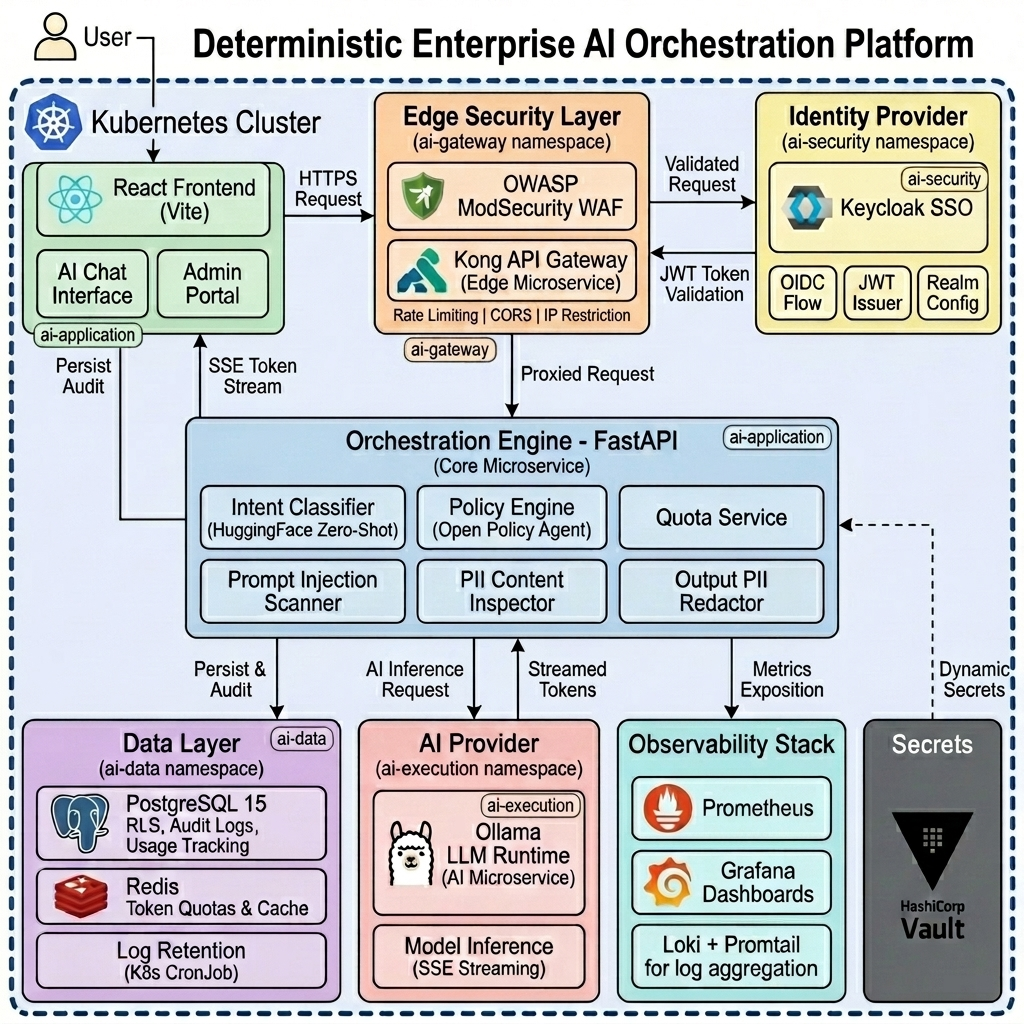
\includegraphics[width=\linewidth,height=\textheight,keepaspectratio]{images/architecture_platform.png}
    \caption{Global Architecture of the Deterministic Enterprise AI Orchestration Platform}
    \label{fig:global_architecture}
    \vfill
\end{figure}
\end{landscape}
\clearpage

\subsection{Kubernetes Deployment Topology}

The architectural topology segregates the platform into independent, scalable microservices orchestrated entirely within Kubernetes:

\begin{figure}[H]
    \centering
    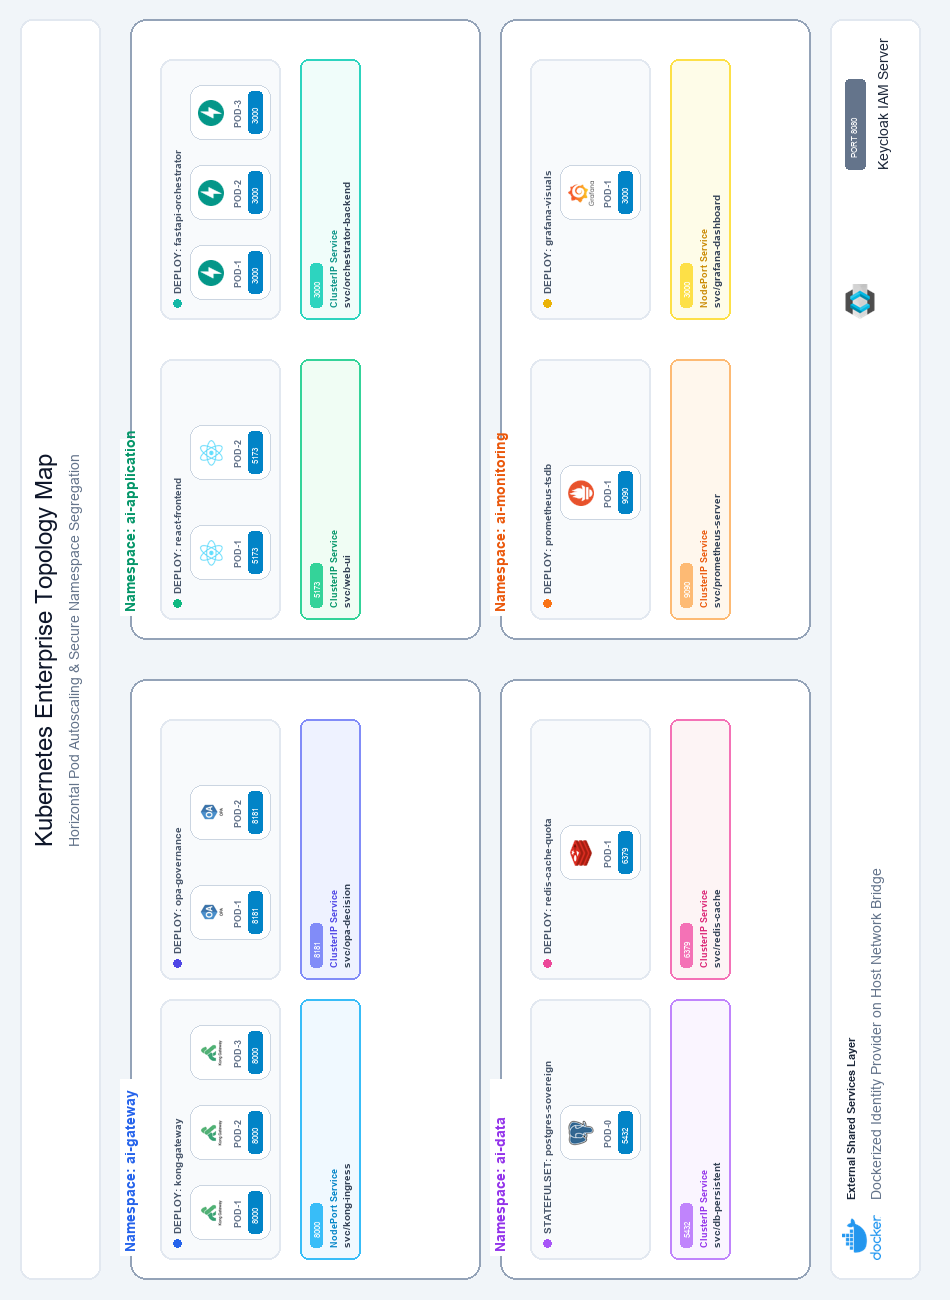
\includegraphics[width=1\textwidth]{images/k8s_architecture_styled.png}
    \caption{Kubernetes Deployment Architecture (\texttt{ai-gateway-namespace})}
    \label{fig:global_system_arch}
\end{figure}

\begin{itemize}
    \item \textbf{Kubernetes Namespace:} The core orchestration engine, API Gateway, and frontend application are securely isolated within the \texttt{ai-gateway-namespace}, ensuring network policies restrict lateral movement.
    \item \textbf{Deployments \& Pods:} Each microservice is managed via a Kubernetes \texttt{Deployment}. As illustrated, the architecture scales horizontally by deploying multiple \textbf{Pods} (e.g., \texttt{POD-1}, \texttt{POD-2}, \texttt{POD-3}) for the Frontend (React), Kong Gateway, and FastAPI backend, guaranteeing high availability.
    \item \textbf{Kubernetes Services:} Traffic is routed to the ephemeral Pods via stable Kubernetes \texttt{Service} abstractions. A \texttt{NodePort} exposes the Kong Gateway for external ingress, while a \texttt{ClusterIP} internally routes authenticated traffic to the FastAPI backend.
    \item \textbf{External Integrations:} Core dependencies such as \textbf{Keycloak} (running as an external Dockerized Identity Provider) and the Data Persistence layers remain highly decoupled from the volatile application workloads.
\end{itemize}

\subsection{Continuous Integration \& Continuous Deployment (CI/CD)}

To ensure absolute stability across iterations, a rigorous Continuous Integration and Continuous Deployment (CI/CD) pipeline was orchestrated via GitHub Actions.

\begin{figure}[H]
    \centering
    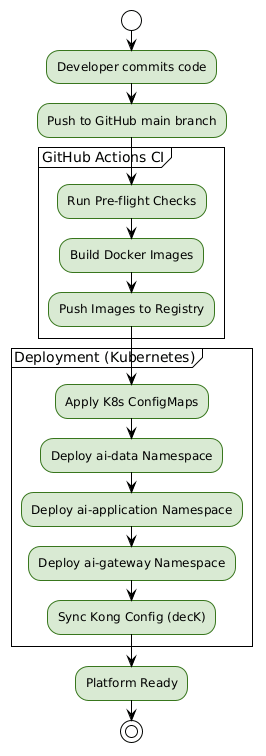
\includegraphics[width=0.25\textwidth]{images/cicd_pipeline.png}
    \caption{CI/CD Pipeline Flow}
    \label{fig:cicd_pipeline}
\end{figure}

Upon every commit to the \texttt{main} branch, the system triggers an automated workflow that executes static analysis (linting, type-checking) and runs the Pytest suite. Upon successful validation, Docker images are built, tagged dynamically, and pushed to a secure registry. Finally, Kubernetes declarative manifests are applied, ensuring zero-downtime rolling updates.

To elevate this deployment process to an enterprise standard, the platform utilizes \textbf{Helm} as its package manager. 

\begin{figure}[H]
    \centering
    
\includegraphics[height=3cm]{images/logos/helm.png}
    \caption{Helm Package Manager Logo}
    \label{fig:helm_logo}
\end{figure}

By packaging all microservices, configurations, and secrets into a unified Helm Chart, the CI/CD pipeline guarantees highly deterministic and repeatable deployments across different environments.

\subsection{Prometheus}

\begin{figure}[H]
    \centering
    
\includegraphics[height=3cm]{images/logos/prometheus.png}
    \caption{Prometheus Logo}
    \label{fig:prometheus_logo}
\end{figure}

Prometheus acts as the central time-series database for the orchestration cluster. It is configured to pull real-time telemetry metrics dynamically from all running Kubernetes Pods, Kong API Gateway endpoints, and FastAPI orchestrator workloads.

\subsection{Grafana}

\begin{figure}[H]
    \centering
    
\includegraphics[height=3cm]{images/logos/grafana.png}
    \caption{Grafana Logo}
    \label{fig:grafana_logo}
\end{figure}

Grafana serves as the visualization and analytical dashboard tier. It connects directly to Prometheus to render rich, interactive dashboards, enabling administrators to monitor real-time token quotas, LLM request latency, and WAF security alerts from a single operational control room.

% ──────────────────────────────────────────────────────────────────
\section*{Conclusion}
\addcontentsline{toc}{section}{Conclusion}
% ──────────────────────────────────────────────────────────────────

This chapter explored the solution's architecture, the open-source technology stack, and the global system topology. We presented the layered microservices architecture, the Kubernetes deployment strategy, and the CI/CD pipeline that ensures continuous delivery. The next chapter will focus on the first release of the project, covering the platform security entry layer and the core orchestration engine.
